\begin{figure}[!b]
	\centering
    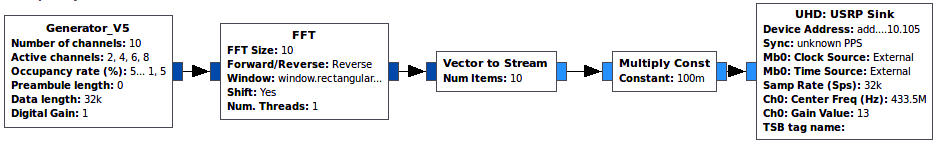
\includegraphics[width=1.00\textwidth]{2-Chapters/4-Chapter/Images/USRP_TX_PU__v1__simple_grc.png}
    \caption[The \textbf{random traffic generator} flow-graph.]{The \textbf{random traffic generator}. \texttt{Generator} is the only hand-written block, which is configured with a list of active channels, a list of occupancy rate, and constants about the PHY layer (preamble length and data length). It uses one USRP only for emitting data (``Sink'' mode).}
    \label{fig:4app:USRP_TX_PU__v1__simple_grc}
\end{figure}

\begin{figure}[!b]
	\centering
    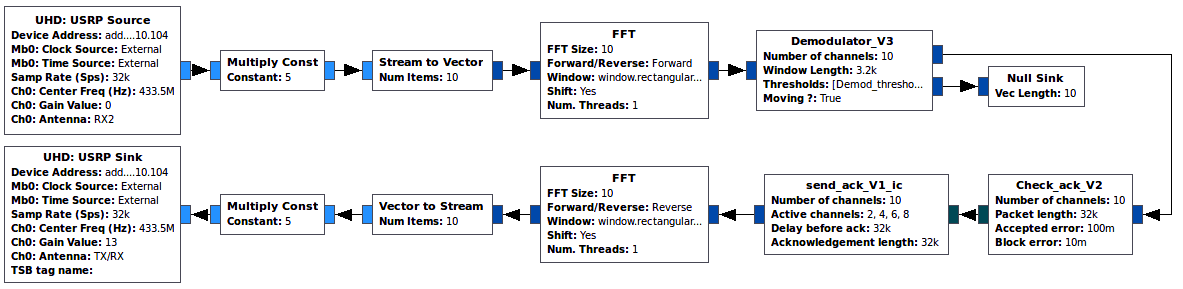
\includegraphics[width=1.00\textwidth]{2-Chapters/4-Chapter/Images/USRP_RX_BTS__v1__simple_grc.png}
    \caption[The \textbf{IoT gateway} flow-graph.]{The \textbf{IoT gateway}. The hand-written blocks are the 1) \texttt{Demodulator} block, which is configured with a list of detection threshold (on the received power), 2) the \texttt{Check\_ack} block, which is configured with a maximum block error and an accepted error rates (to decide when a message is close enough to an acknowledgement), and finally 3) the \texttt{send\_ack} block, which is configured with the list of active channels, and knowledge about the PHY layer (delay before sending the Ack and its length). All blocks need to know constants about the PHY layer (preamble length and data length). The IoT gateway uses one USRP for both emitting and receiving data (``Sink'' and ``Source'' modes).}
    \label{fig:4app:USRP_RX_BTS__v1__simple_grc}
\end{figure}

\begin{figure}[!b]
	\centering
    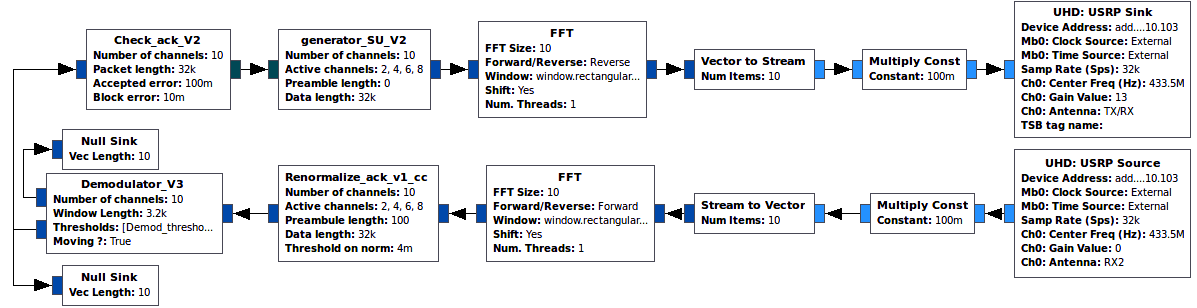
\includegraphics[width=1.00\textwidth]{2-Chapters/4-Chapter/Images/USRP_TX_SU__v1__simple_grc.png}
    \caption[The \textbf{IoT dynamic device} flow-graph.]{The \textbf{IoT dynamic device}. The hand-written blocks are the 1) the \texttt{Renormalized\_ack} block, which is configured with the list of active channels and extra knowledge about the PHY layer (preamble length, message length, and a threshold to tune detection of the incoming Ack), 2) the \texttt{Demodulator} and 3) the \texttt{Check\_ack} blocks, both shared with the IoT gateway, and finally 4) the \texttt{generator\_SU} block, which embeds the \UCB{} or Thompson Sampling algorithm, and which is configured with the list of active channels. Most blocks need to know constants about the PHY layer (preamble length and data length). Any of the IoT dynamic devices use one USRP for both emitting and receiving data (``Sink'' and ``Source'' modes).}
    \label{fig:4app:USRP_TX_SU__v1__simple_grc}
\end{figure}